\documentclass[11pt,a4paper]{article}
\ifdefined\pdfsuppresswarningpagegroup
  \pdfsuppresswarningpagegroup=1
\fi

% ------------------------------------------------------------
% Packages
% ------------------------------------------------------------
\usepackage[utf8]{inputenc}
\usepackage[T1]{fontenc}
\usepackage{amsmath,amssymb,amsfonts}
\usepackage{graphicx}
\usepackage{booktabs}
\usepackage[hidelinks]{hyperref}
\usepackage{geometry}
\usepackage{authblk}
\usepackage{bm}
\usepackage{caption}
\usepackage{subcaption}
\usepackage{microtype}
\usepackage{xcolor}
\usepackage{float}

\geometry{margin=1in}
\setlength{\emergencystretch}{2em}

% Use the real figure when available; otherwise insert a visible placeholder.
% This keeps the manuscript compilable when the source is shared without the figure directory.
\newcommand{\safeincludegraphics}[2][]{%
  \IfFileExists{#2}{%
    \includegraphics[#1]{#2}%
  }{%
    \fbox{%
      \parbox[c][4.2cm][c]{0.88\linewidth}{%
        \centering Missing figure file:\\[4pt]
        \footnotesize\nolinkurl{#2}%
      }%
    }%
  }%
}


% ------------------------------------------------------------
% Title
% ------------------------------------------------------------
\title{
Shortest-Path Anisotropy in Black-Hole Embedding Graphs:\\
Geometric Organization and Construction Sensitivity
}

\author[1]{Ariadna Uxue Palomino Ylla}
\affil[1]{Department of Physics, Nagoya University, Nagoya, Japan}

\date{}

% ------------------------------------------------------------
% Document
% ------------------------------------------------------------
\begin{document}

\maketitle

\begin{abstract}
Shortest-path observables on geometric graphs can display clear organization inherited from an underlying sampled space, but their values can also depend strongly on sampling, edge construction, graph scale, and the chosen null model. We study this tension using graph discretizations of embedded spatial slices of static black-hole geometries. Our diagnostic, $C_{\log}$, is the cubic mean deviation of logarithmic shortest-path multiplicities over finite graph-distance shells.

We perform a paired ten-seed Schwarzschild/Flamm audit using five graph/control protocols: the original matched-flat KNN convention, strict radius-threshold controls, pure KNN graphs, mutual KNN graphs, and edge-count-matched radius graphs. For each protocol we correlate the radial coordinate with common-bin mean $C_{\log}$ profiles and compare the black-hole and flat-control correlations. Mean absolute gaps range from $0.233\pm0.199$ for pure KNN to $0.688\pm0.442$ for strict radius (mean $\pm$ standard deviation). Signed gaps change sign for some seeds and protocols, while strict-radius and edge-matched protocols give the largest average magnitudes.

The black-hole/control separation is therefore neither graph-construction invariant nor realization independent. Its magnitude and sign depend on the complete diagnostic--construction--control protocol. $C_{\log}$ is a reproducible finite-graph statistic under specified conditions, but the present evidence does not support interpreting it as a graph-independent curvature scalar. Reissner--Nordstr\"om, Bardeen, Hayward, graph-curvature baselines, and non-black-hole surfaces remain important benchmark families, but their earlier numerical tables are excluded here because the corresponding raw data were not available for reconciliation with the canonical common-bin pipeline.
\end{abstract}

\section{Introduction}
\label{sec:introduction}

The problem of representing curvature in discrete spaces has a long history, from Regge calculus \cite{Regge1961} to modern notions of graph and cell-complex curvature \cite{Forman2003,Ollivier2009,JostLiu2014}. Geometric graphs are also widely used as finite representations of sampled metric spaces, spatial data, and data-driven geometries \cite{Penrose2003,DallChristensen2002,Newman2010}. In a graph, however, there is no unique analogue of continuum curvature. Different constructions probe different features, including transport contraction, cell incidence, neighborhood growth, clustering, and shortest-path structure.

A second difficulty is that a graph observable is rarely a function of the sampled geometry alone. It can also depend on sampling density, boundary treatment, edge rule, graph scale, and the null model used for comparison. Related problems are well known in thresholded and density-controlled network analyses, where changing the graph construction can change the interpretation of a measured statistic \cite{VanWijk2010,Langer2013,Ginestet2011}. Consequently, a convincing geometric interpretation requires both positive benchmark evidence and a construction-matched stress test.

Here we study a shell-based shortest-path anisotropy statistic, $C_{\log}$, defined from the dispersion of logarithmic shortest-path multiplicities between a reference vertex and vertices on a finite graph-distance shell. The primary testbeds are Euclidean embeddings of equatorial spatial slices of Schwarzschild/Flamm, Reissner--Nordstr\"om, Bardeen, and Hayward geometries. These surfaces provide smooth, radially organized benchmarks with known continuum curvature profiles.

The quantitative part of this paper asks how the Schwarzschild/Flamm signal changes with graph construction and control matching. We compare the original protocol with strict radius-threshold controls, pure KNN graphs, mutual KNN graphs, and edge-count-matched radius graphs over the same ten paired point samples. The result is not a monotone ``correction'' toward zero: radius-style protocols have the largest mean absolute separation, whereas the original and pure-KNN protocols have smaller and less sign-stable gaps.

The broader Reissner--Nordstr\"om, Bardeen, Hayward, logarithmic-Kretschmann, Forman--Ricci, Ollivier--Ricci, and non-black-hole benchmark programs remain scientifically useful. A provenance audit found, however, that their legacy numerical tables mixed vertex-level or legacy seed-level conventions with the newer common-bin profile convention, and their raw rows were not included in the available repository. We retain their geometry definitions and validation role but do not treat their old point estimates as current evidence.

The central claim is therefore deliberately narrower than a universal curvature-estimator claim. The statistic is a finite-shell diagnostic of shortest-path multiplicity organization whose meaning is defined by the complete diagnostic--construction--control triple. The matched-control audit is not an afterthought: it determines the domain in which the positive benchmark signal can be interpreted.

The paper is organized as follows. Section~\ref{sec:estimator} defines $C_{\log}$. Section~\ref{sec:geometries} introduces the embedding geometries, graph protocol, controls, and numerical conventions. Sections~\ref{sec:results-schwarzschild}--\ref{sec:results-regular} define the broader benchmark program and its provenance status. Section~\ref{sec:construction-audit} gives the audited Schwarzschild analysis. Section~\ref{sec:baselines} discusses graph-curvature baselines, and Section~\ref{sec:limitations} gives scope and limitations. Sections~\ref{sec:discussion} and \ref{sec:conclusion} state the interpretation.

\section{Graph-shell path-anisotropy statistic}
\label{sec:estimator}

Let $G=(V,E)$ be a finite, undirected graph. For two vertices $p,q\in V$, let $d_G(p,q)$ denote graph distance, i.e. the length of the shortest path between $p$ and $q$. For a reference vertex $p$ and an integer graph radius $r_g$, define the graph-distance shell
\begin{equation}
    S_{r_g}(p)
    =
    \{q\in V : d_G(p,q)=r_g\}.
\end{equation}
Let
\begin{equation}
    N_{\mathrm{geo}}(p,q)
\end{equation}
denote the number of distinct shortest paths from $p$ to $q$. We define the logarithmic shortest-path multiplicity variable
\begin{equation}
    X_{p,q}
    =
    \log N_{\mathrm{geo}}(p,q),
    \qquad q\in S_{r_g}(p).
\end{equation}
The path-anisotropy estimator used in this work is the cubic mean deviation of $X_{p,q}$ over the shell:
\begin{equation}
    C_{\log}(p,r_g)
    =
    \left[
    \frac{1}{|S_{r_g}(p)|}
    \sum_{q\in S_{r_g}(p)}
    \left|
    X_{p,q}
    -
    \overline{X}_{p,r_g}
    \right|^3
    \right]^{1/3},
    \label{eq:clog}
\end{equation}
where
\begin{equation}
    \overline{X}_{p,r_g}
    =
    \frac{1}{|S_{r_g}(p)|}
    \sum_{q\in S_{r_g}(p)}
    X_{p,q}.
\end{equation}

The quantity $C_{\log}$ is not proposed as a universal discrete curvature scalar. Instead, it measures the anisotropy of shortest-path multiplicities over a finite graph-distance shell. Its value depends on graph construction, sampling, and shell radius. The central question of this paper is whether, under a fixed graph construction and matched-control convention, $C_{\log}$ detects curvature-organized structure in graph discretizations of black-hole embedding geometries.

\section{Black-hole embedding geometries and graph construction}
\label{sec:geometries}

\subsection{Static spherical backgrounds}

We consider static, spherically symmetric metrics of the form
\begin{equation}
    ds^2
    =
    -f(r)dt^2
    +
    f(r)^{-1}dr^2
    +
    r^2d\Omega^2.
\end{equation}
On an equatorial spatial slice,
\begin{equation}
    dl^2=f(r)^{-1}dr^2+r^2d\phi^2.
\end{equation}
Embedding the slice as a surface of revolution in Euclidean three-space gives
\begin{equation}
    \frac{dz}{dr}=\sqrt{\frac{1}{f(r)}-1}.
    \label{eq:embedding}
\end{equation}
We consider the following black-hole families.

\paragraph{Schwarzschild.}
For Schwarzschild \cite{Schwarzschild1916,Flamm1916},
\begin{equation}
    f_{\mathrm{Schw}}(r)
    =
    1-\frac{2M}{r}.
\end{equation}
The Kretschmann scalar is
\begin{equation}
    K_{\mathrm{Schw}}(r)
    =
    \frac{48M^2}{r^6}.
\end{equation}

\paragraph{Reissner--Nordstr\"om.}
For Reissner--Nordstr\"om \cite{Reissner1916,Nordstrom1918},
\begin{equation}
    f_{\mathrm{RN}}(r)
    =
    1-\frac{2M}{r}
    +
    \frac{Q^2}{r^2}.
\end{equation}
The Kretschmann scalar is
\begin{equation}
    K_{\mathrm{RN}}(r)
    =
    \frac{48M^2}{r^6}
    -
    \frac{96MQ^2}{r^7}
    +
    \frac{56Q^4}{r^8}.
    \label{eq:rnK}
\end{equation}

\paragraph{Bardeen.}
For the Bardeen regular black-hole family \cite{Bardeen1968}, we use
\begin{equation}
    m_{\mathrm{B}}(r)
    =
    \frac{Mr^3}{(r^2+g^2)^{3/2}},
\end{equation}
so that
\begin{equation}
    f_{\mathrm{B}}(r)
    =
    1-\frac{2m_{\mathrm{B}}(r)}{r}
    =
    1-\frac{2Mr^2}{(r^2+g^2)^{3/2}}.
\end{equation}

\paragraph{Hayward.}
For the Hayward regular black-hole family \cite{Hayward2006}, we use
\begin{equation}
    m_{\mathrm{H}}(r)
    =
    \frac{Mr^3}{r^3+2M\ell^2},
\end{equation}
so that
\begin{equation}
    f_{\mathrm{H}}(r)
    =
    1-\frac{2m_{\mathrm{H}}(r)}{r}
    =
    1-\frac{2Mr^2}{r^3+2M\ell^2}.
\end{equation}

For a metric of the above form, the Kretschmann scalar can be computed from $f(r)$ as
\begin{equation}
    K(r)
    =
    \left(f''(r)\right)^2
    +
    \left(\frac{2f'(r)}{r}\right)^2
    +
    \frac{4(1-f(r))^2}{r^4}.
    \label{eq:kfromf}
\end{equation}
In the numerical implementation, this formula is evaluated analytically for Schwarzschild and Reissner--Nordstr\"om. For the Bardeen and Hayward scans, it is evaluated by numerical differentiation of $f(r)$.

\subsection{Graph construction}

Each embedded geometry is represented by a finite point cloud on the embedded surface. The points are sampled using a radial-angular prescription calibrated on the Schwarzschild/Flamm case. The graph is then built from the embedded coordinates using a geometric graph construction. Its length scale is selected from a distance-matrix radius rule controlled by $k$. Unless otherwise stated, we use $N=1000$, $k=16$, and graph-shell radius $r_g=3$.

The matched-flat control is built from the same radial and angular samples but with the height profile removed:
\begin{equation}
    (r,\phi,z(r))
    \longrightarrow
    (r,\phi,0).
\end{equation}
This control tests whether the observed radial organization of $C_{\log}$ is explained purely by the radial sampling, rather than by the embedded black-hole geometry.

A crucial point is that the diagnostic is sensitive to graph construction. In the original calibrated comparison, the black-hole graph is generated with the radius-threshold construction, whereas the original matched-flat control uses a matched-flat KNN convention. That pairing produced the motivating separation, but it also makes the construction/control choice part of the hypothesis being tested. We therefore treat the edge rule and null model as explicit components of the experimental protocol and later repeat the comparison with symmetrically constructed controls.

The conclusions below should be read as statements about specified finite-graph protocols, not as claims of a graph-independent continuum invariant.

\subsection{Numerical protocol and correlation conventions}
\label{sec:numerical-protocol}

Unless otherwise stated, the benchmark graphs use $N=1000$ sampled vertices, construction parameter $k=16$, graph-shell radius $r_g=3$, and 12 radial bins. The black-hole graph and its matched controls use common radial-angular samples. Vertex-level values are evaluated first and then aggregated when radial profiles are required.

The canonical quantitative pipeline in this revision is the construction audit. For each seed and protocol, vertex-level $C_{\log}$ values are computed first. The black-hole and flat results are then passed, in that order, to a common radial-binning routine. Pearson correlations are computed between the common-bin mean radius and the common-bin mean $C_{\log}$ profile. Thus $\rho_r(C_{\log})_{\mathrm{BH}}$ and $\rho_r(C_{\log})_{\mathrm{flat}}$ use identical bins, and
\begin{equation}
\Delta\rho_r=\rho_r(C_{\log})_{\mathrm{BH}}-\rho_r(C_{\log})_{\mathrm{flat}}.
\end{equation}
No sign reversal to $-C_{\log}$ is used. Legacy vertex-level and seed-level correlations are not combined numerically with this common-bin statistic. The complete mapping of manuscript results to code and data is provided in the machine-readable provenance table distributed with the repository.

\section{Schwarzschild/Flamm calibration}
\label{sec:results-schwarzschild}

The Schwarzschild/Flamm embedding is the primary audited benchmark. The paired design uses $M=1/2$, $N=1000$, $k=16$, $r_g=3$, 12 common radial bins, and seeds 1 through 10. Each seed generates one Flamm point sample, and all five protocols reuse its radial-angular coordinates. All 50 graph pairs passed pairing, connectivity, estimator-validity, mutual-KNN, and edge-matching checks. Section~\ref{sec:construction-audit} reports the protocol-specific correlations and uncertainties.

Earlier calibration values were based on a legacy seed-level convention and were not accompanied by stored raw rows. They are therefore not combined with, or used to validate, the common-bin construction audit. This distinction explains why the signs and magnitudes in older calibration tables can differ substantially from the canonical values below without implying an arithmetic contradiction.

\section{Reissner--Nordstr\"om charge scan}
\label{sec:results-rn}

The Reissner--Nordstr\"om family provides the natural charged extension of the benchmark. The implemented scan uses $M=1/2$ and
\begin{equation}
    Q=0,0.1,0.2,0.3,0.4.
\end{equation}
The extremal value is $Q=M=0.5$, so $Q=0.4$ is already a near-extremal deformation within this parameterization.

The code constructs these embeddings and their Kretschmann profiles, but the raw seed-level rows behind the previous charge table and figure were not supplied. Those legacy correlations also used a seed-level convention that is incompatible with the canonical common-bin construction audit. The old point estimates and figure are therefore removed rather than silently reinterpreted. A publishable RN claim requires a new paired, common-bin, multi-protocol rerun; its status is recorded as ``rerun required'' in the provenance table.

\section{Regular black-hole scans: Bardeen and Hayward}
\label{sec:results-regular}

We now test two regular black-hole families: Bardeen and Hayward. In both cases, the zero-parameter limit reduces to Schwarzschild, providing a consistency check. The scans use
\begin{equation}
    g=0,0.1,0.2,0.3
\end{equation}
for Bardeen and
\begin{equation}
    \ell=0,0.1,0.2,0.3
\end{equation}
for Hayward, again with $M=1/2$, $N=1000$, $k=16$, $r_g=3$, and ten random seeds.

\subsection{Bardeen scan}

The Bardeen builder and numerical Kretschmann calculation are retained in the package, including the Schwarzschild limit $g=0$. The earlier parameter table and figure are not retained as evidence because neither their raw seed rows nor their exact bin assignments are available. A future rerun must use the same paired common-bin conventions as the audited Schwarzschild calculation.

\subsection{Hayward scan}

The Hayward builder is likewise retained, with $\ell=0$ as the Schwarzschild limit. Its legacy table and figure have the same provenance gap as the Bardeen scan and are removed pending a paired common-bin rerun. Consequently, the present manuscript does not claim cross-family numerical robustness; it identifies RN, Bardeen, and Hayward as preregistered extension families for the audited protocol.

\subsection{Cross-family profiles under the binned-profile convention}
\label{sec:cross-family-profiles}

Cross-family comparisons are especially vulnerable to pipeline mixing because a vertex-level $\mathrm{Corr}(r,C_{\log})$, a correlation of independently binned profiles, and a correlation of BH/flat common-bin profiles are different statistics. The former manuscript combined signs from more than one of these conventions. Because the underlying profiles are unavailable, the cross-family table and figures are removed. The implemented geometries and Kretschmann functions remain in the code so that RN, Bardeen, and Hayward can later be rerun under a single preregistered common-bin protocol.


\section{Construction-sensitivity audit}
\label{sec:construction-audit}

The audit asks whether the Schwarzschild/Flamm black-hole/control separation is invariant when the edge rule and control construction change. It is a paired experiment: a seed generates the Flamm sample exactly once, every control preserves its radial-angular sample, and all five protocols reuse that sample. The calibrated radius convention retains the factor 1.15. Every graph retains all 1000 vertices, including isolates; in the observed runs all graphs were connected and every valid-$C_{\log}$ fraction was one.

We consider five protocols:
\begin{enumerate}
    \item the original matched-flat KNN protocol;
    \item a strict radius-threshold matched-flat control;
    \item pure KNN graphs for both the black-hole geometry and the flat control;
    \item mutual KNN graphs for both the black-hole geometry and the flat control;
    \item edge-count-matched radius graphs for both the black-hole geometry and
    the flat control.
\end{enumerate}

For each protocol the same common-bin implementation produces $\rho_r(C_{\log})_{\mathrm{BH}}$ and $\rho_r(C_{\log})_{\mathrm{flat}}$. We report signed $\Delta\rho_r$ to retain direction and $|\Delta\rho_r|$ to summarize separation magnitude. Means and uncertainty are computed across the ten paired seeds.

\begin{table}[H]
\centering
\caption{
Summary of the graph-construction and matched-control protocols used in the
construction-sensitivity audit.
}
\label{tab:protocol-summary}
\small
\setlength{\tabcolsep}{4pt}
\resizebox{\linewidth}{!}{%
\begin{tabular}{lll}
\toprule
Protocol & Black-hole graph & Flat control \\
\midrule
Original matched-flat KNN
& Radius-threshold graph
& Matched-flat KNN graph \\
Strict radius
& Radius-threshold graph
& Matched-flat radius-threshold graph \\
Pure KNN
& KNN graph
& KNN graph \\
Mutual KNN
& Mutual-KNN graph
& Mutual-KNN graph \\
Edge-matched radius
& Calibrated radius-threshold graph
& Edge-count-matched radius graph \\
\bottomrule
\end{tabular}%
}
\end{table}

\begin{table}[H]
\centering
\caption{Ten-seed Schwarzschild/Flamm construction audit. Values are mean $\pm$ standard deviation. Signed and absolute gaps are reported separately.}
\label{tab:construction-summary}
\small
\begin{tabular}{lcc}
\toprule
Protocol & Signed $\Delta\rho_r$ & $|\Delta\rho_r|$ \\
\midrule
Original matched-flat KNN & $0.160\pm0.250$ & $0.242\pm0.161$ \\
Strict radius             & $0.688\pm0.442$ & $0.688\pm0.442$ \\
Pure KNN                  & $-0.189\pm0.245$ & $0.233\pm0.199$ \\
Mutual KNN                & $0.392\pm0.362$ & $0.422\pm0.323$ \\
Edge-matched radius       & $0.681\pm0.445$ & $0.681\pm0.445$ \\
\bottomrule
\end{tabular}
\end{table}

\begin{table}[H]
\centering
\caption{Detailed uncertainty for the mean absolute gap. The confidence interval is a two-sided Student-$t$ interval for the mean with nine degrees of freedom.}
\label{tab:construction-detail}
\small
\resizebox{\linewidth}{!}{%
\begin{tabular}{lccccc}
\toprule
Protocol & Mean $|\Delta\rho_r|$ & SEM & 95\% CI & Minimum & Maximum \\
\midrule
Original matched-flat KNN & 0.242 & 0.051 & [0.126, 0.357] & 0.078 & 0.610 \\
Strict radius             & 0.688 & 0.140 & [0.372, 1.005] & 0.114 & 1.362 \\
Pure KNN                  & 0.233 & 0.063 & [0.091, 0.375] & 0.020 & 0.526 \\
Mutual KNN                & 0.422 & 0.102 & [0.192, 0.653] & 0.056 & 1.013 \\
Edge-matched radius       & 0.681 & 0.141 & [0.363, 1.000] & 0.112 & 1.313 \\
\bottomrule
\end{tabular}%
}
\end{table}

\begin{figure}[H]
\centering
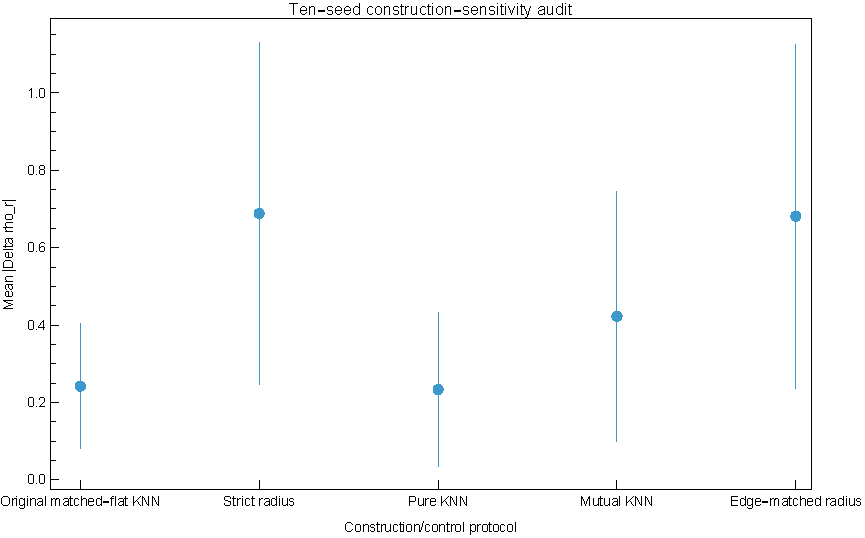
\includegraphics[width=0.86\linewidth]{results/construction_audit_multiseed/schwarzschild_five_protocols_N1000_seeds10_mean_sd.pdf}
\caption{Mean absolute radial-correlation gap across ten paired seeds. Error bars show standard deviation, not standard error. Radius-style protocols have the largest marginal means, but the broad seed-to-seed variation motivates paired analysis.}
\label{fig:construction-summary}
\end{figure}

\subsection{Seed-level distributions and paired contrasts}

The median absolute gaps are 0.240 (original), 0.628 (strict radius), 0.140 (pure KNN), 0.302 (mutual KNN), and 0.630 (edge-matched radius). The corresponding interquartile ranges are 0.215, 0.764, 0.389, 0.541, and 0.770. Figure~\ref{fig:paired-abs} shows that the protocols are paired through the same realizations and that their ordering varies by seed.

\begin{figure}[H]
\centering
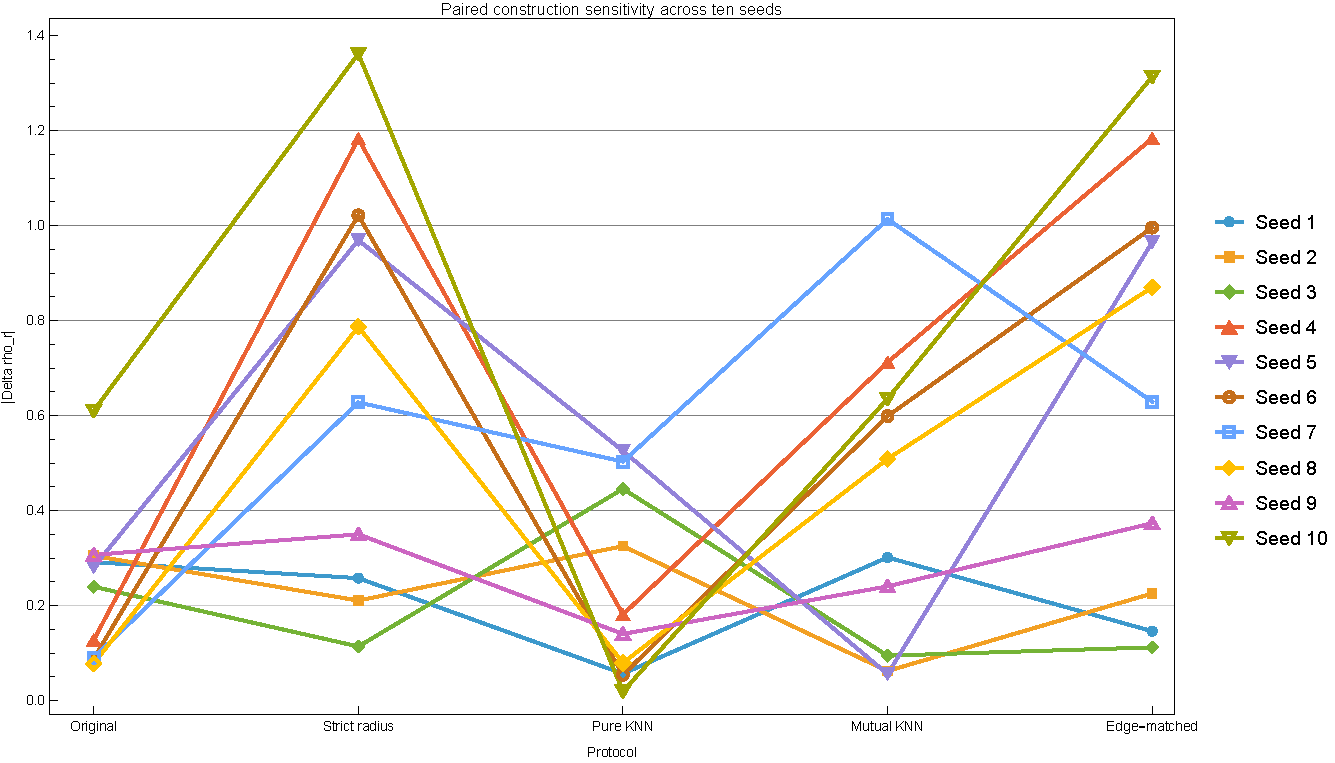
\includegraphics[width=0.94\linewidth]{results/construction_audit_multiseed/seed_level_analysis/paired_abs_delta_by_seed.pdf}
\caption{Paired $|\Delta\rho_r|$ values for all ten seeds. Lines connect the same Flamm point sample across protocols. The plot displays realization dependence directly; it is not a collection of independent protocol samples.}
\label{fig:paired-abs}
\end{figure}

\begin{figure}[H]
\centering
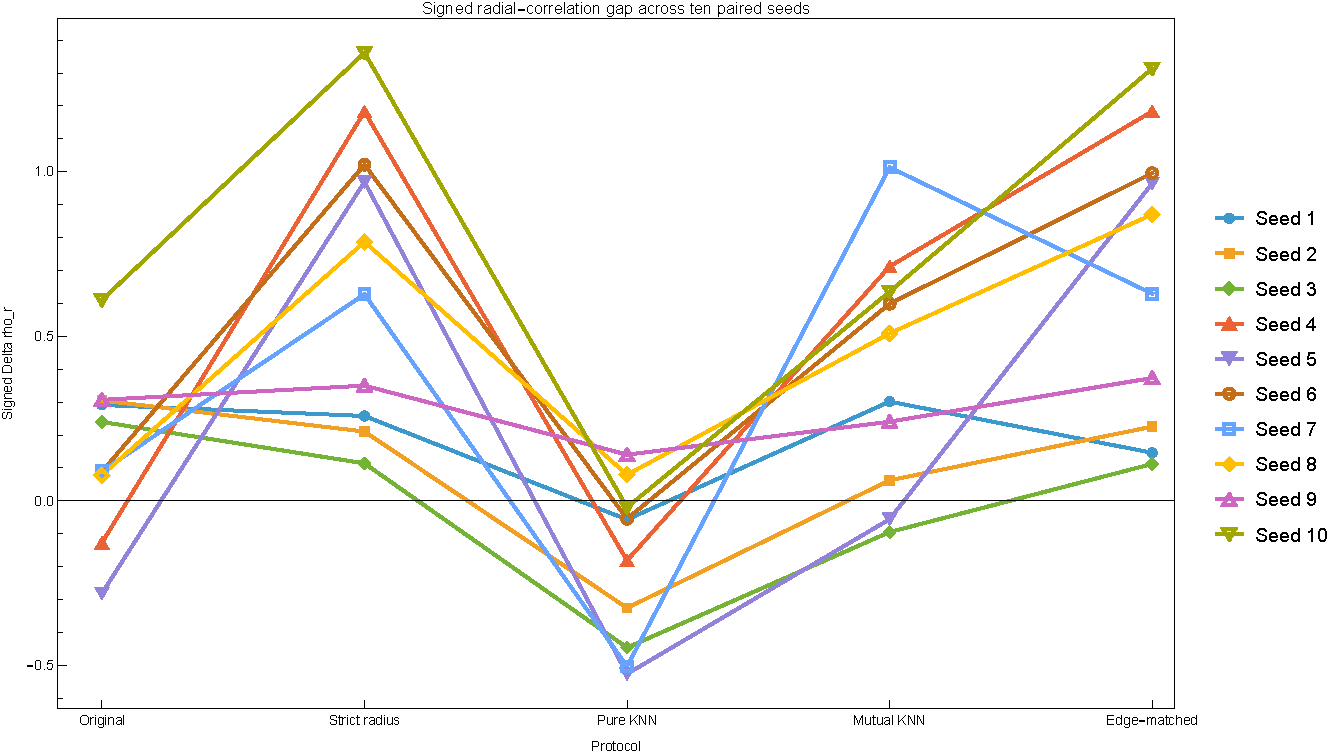
\includegraphics[width=0.94\linewidth]{results/construction_audit_multiseed/seed_level_analysis/paired_signed_delta_by_seed.pdf}
\caption{Signed $\Delta\rho_r$ for the same paired realizations. Original, pure-KNN, and mutual-KNN protocols change sign for some seeds, whereas strict-radius and edge-matched-radius gaps are positive in all ten audited runs.}
\label{fig:paired-signed}
\end{figure}

Table~\ref{tab:paired-contrasts} reports selected paired differences in absolute gap. Strict radius exceeds the original protocol by 0.446 on average and pure KNN by 0.455; edge-matched radius gives similar contrasts. Strict radius and edge-matched radius are nearly indistinguishable in this sample. Original and pure KNN also have a near-zero mean paired contrast. These intervals describe paired mean differences without claiming a definitive protocol ranking at $N=10$. In particular, overlap of the marginal confidence intervals in Table~\ref{tab:construction-detail} is not a paired significance test.

\begin{table}[H]
\centering
\caption{Paired contrasts in $|\Delta\rho_r|$. The contrast is protocol A minus protocol B; intervals are two-sided Student-$t$ intervals over ten paired seeds.}
\label{tab:paired-contrasts}
\small
\resizebox{\linewidth}{!}{%
\begin{tabular}{llcc}
\toprule
Protocol A & Protocol B & Mean paired difference & 95\% CI \\
\midrule
Original & Strict radius       & $-0.446$ & [$-0.771,-0.122$] \\
Original & Pure KNN            & $0.009$  & [$-0.192,0.209$] \\
Original & Mutual KNN          & $-0.181$ & [$-0.468,0.107$] \\
Original & Edge-matched radius & $-0.440$ & [$-0.771,-0.108$] \\
Strict radius & Pure KNN       & $0.455$  & [$0.071,0.839$] \\
Strict radius & Mutual KNN     & $0.266$  & [$-0.008,0.540$] \\
Strict radius & Edge-matched radius & $0.007$ & [$-0.029,0.043$] \\
Pure KNN & Mutual KNN          & $-0.189$ & [$-0.484,0.106$] \\
Pure KNN & Edge-matched radius & $-0.448$ & [$-0.831,-0.066$] \\
Mutual KNN & Edge-matched radius & $-0.259$ & [$-0.535,0.017$] \\
\bottomrule
\end{tabular}%
}
\end{table}

The audit therefore rejects both graph-construction invariance and realization independence. Radius-style protocols produce the largest mean absolute separation in this Schwarzschild benchmark, while the original and pure-KNN protocols give smaller and less sign-stable gaps. This is a statement about the specified finite-graph experiment, not a universal ordering of graph constructions.

\section{Comparison with graph-curvature baselines}
\label{sec:baselines}

Forman--Ricci curvature \cite{Forman2003} and Ollivier--Ricci curvature \cite{Ollivier2009} remain important comparators because they probe local incidence and neighborhood transport rather than shortest-path multiplicity. The legacy manuscript reported single-realization vertex-level correlations for both baselines, but neither the raw vertex scores nor the source figures are present in the supplied repository.

The legacy Forman calculation averaged unweighted edge scores at vertices, but its source rows are absent and its vertex-level correlation is not the common-bin statistic used here.

The legacy Ollivier calculation has the same provenance limitation. A valid baseline comparison must apply both curvatures to the same ten point samples, state whether edge or vertex curvature is correlated, use construction-matched controls, and report vertex-level and common-bin results without mixing signs. Until that rerun is completed, the baselines define future controls rather than evidence that $C_{\log}$ outperforms or duplicates a standard graph curvature.

\section{Additional benchmark surfaces and scope}
\label{sec:limitations}

Sphere caps, hyperbolic disks, paraboloids, and hyperbolic paraboloids remain useful non-black-hole test surfaces because they separate constant curvature, radial curvature variation, and saddle-like geometry. The legacy manuscript contained qualitative claims about these surfaces but no raw rows, construction matrix, or source figures. Those claims are removed from the present evidence set. A future benchmark should reuse the paired multi-protocol design and report boundary handling explicitly.

The main limitations are therefore:
\begin{enumerate}
    \item \textbf{Construction and null-model dependence.} The edge rule and matched-control convention change both the magnitude and, for some protocols and seeds, the sign of the separation.

    \item \textbf{Finite-shell character.} The statistic is evaluated at finite graph radius $r_g$ and is affected by graph size, shell occupancy, boundaries, and binning. It is not a pointwise continuum invariant.

    \item \textbf{Correlation is not identification.} A strong association between $C_{\log}(r)$ and $\log K(r)$ within one protocol does not by itself establish that $C_{\log}$ estimates the Kretschmann scalar; both can share a radial trend.

    \item \textbf{Embedding-specific interpretation.} The present graphs are built from Euclidean embeddings of spatial slices. The relation to intrinsic two-dimensional curvature, four-dimensional spacetime curvature, or non-embeddable data requires separate analysis.

    \item \textbf{Incomplete broader benchmark provenance.} RN, Bardeen, Hayward, Forman--Ricci, Ollivier--Ricci, and non-black-hole surfaces have not yet been subjected to the same stored-raw-data, multi-protocol audit as the Schwarzschild benchmark.

    \item \textbf{Small seed sample.} Ten paired seeds reveal substantial realization variability but give broad uncertainty intervals. Marginal means should not be treated as a definitive ranking of protocols.
\end{enumerate}

These limitations distinguish three claims that are often conflated: reproducibility within a fixed protocol, sensitivity across graph-construction protocols, and graph-independent curvature invariance. The first can be quantified only together with realization variability; the second is directly observed; the third is not supported.

\section{Discussion}
\label{sec:discussion}

The paired audit resolves the apparent tension in the legacy construction claims by showing that the old single-realization values were not representative of the canonical ten-seed common-bin pipeline. The Schwarzschild black-hole/control separation varies substantially across seeds and protocols. Strict-radius and edge-matched-radius controls do not reduce the mean gap to $10^{-3}$; instead they give the largest mean absolute gaps, $0.688\pm0.442$ and $0.681\pm0.445$, respectively. The original and pure-KNN means are smaller, $0.242\pm0.161$ and $0.233\pm0.199$, and their signed gaps are less stable.

Reproducibility within a protocol is not graph-construction invariance. The seed-level lines show that the same point realization can move markedly when its edge rule or control changes. The paired contrasts further show that strict radius and edge-matched radius are nearly indistinguishable in this sample, whereas both exceed original and pure KNN in several paired comparisons. With only ten seeds, these results support protocol sensitivity but not a universal ranking.

This result changes the interpretation rather than making the original computation meaningless. $C_{\log}$ measures dispersion in finite-shell shortest-path multiplicities. Those multiplicities are determined jointly by the sampled geometry and by the graph representation imposed on it. The appropriate object of interpretation is therefore
\begin{equation}
    \text{diagnostic} \; + \; \text{construction} \; + \; \text{control},
\end{equation}
not the diagnostic in isolation.

The provenance audit also prevents a different overclaim: legacy Forman--Ricci, Ollivier--Ricci, cross-family, and non-black-hole values cannot be used to rank diagnostics because their raw data and exact correlation pipelines are absent. They remain necessary future comparators, but not supporting numerical evidence in this revision.

A practical consequence is a reporting standard for future geometric-graph studies. Alongside the diagnostic definition, one should report the sampling prescription, edge rule, edge density or scale, shell radius, boundary handling, radial binning, and null-model construction. At minimum, a claim of geometric sensitivity should be tested against (i) a sampling-matched control, (ii) a construction-matched control, and (iii) an edge-count- or density-matched control. Multi-seed and multi-resolution tests should then distinguish stochastic stability from continuum convergence.

Several extensions would materially strengthen the result. The audit should be repeated across graph sizes, shell radii, and radial-bin choices. RN, Bardeen, Hayward, Forman--Ricci, Ollivier--Ricci, and non-black-hole surfaces should be audited under the same paired construction matrix with stored raw rows. Partial-correlation or residual analyses controlling for radial coordinate, degree, edge length, and shell size would help identify what information remains beyond generic radial organization.

Within these limits, the positive conclusion is precise: $C_{\log}$ is a reproducible finite-graph statistic when sampling, construction, control, shell radius, binning, and seed are specified. The negative conclusion is equally important: it is not a graph-independent discrete Kretschmann scalar.

\section{Conclusion}
\label{sec:conclusion}

We studied the shell-based shortest-path anisotropy statistic $C_{\log}$ on Schwarzschild/Flamm geometric graphs through a paired ten-seed, five-protocol construction audit. The black-hole/control separation is neither graph-construction invariant nor realization independent. Its magnitude and sign depend on the full diagnostic--construction--control protocol. Radius-style protocols produce the largest mean absolute separation in this audit, while the original and pure-KNN protocols give smaller and less sign-stable gaps.

The correct conclusion is not that $C_{\log}$ universally reconstructs curvature. It is a finite-shell graph statistic that can be reproduced under fully specified conditions, but its discriminatory power depends on the graph representation and null model. The paired audit separates three questions: stochastic reproducibility within a protocol, sensitivity across protocols, and graph-independent curvature invariance. The data quantify the first two and do not support the third.

RN, Bardeen, Hayward, logarithmic-Kretschmann comparisons, Forman--Ricci and Ollivier--Ricci baselines, and non-black-hole surfaces remain essential extensions. Their earlier numerical claims require regeneration under the canonical stored-raw-data pipeline before they can support the paper's conclusions.

\section*{Code and data availability}

The code, notebooks, tables, and figures used in this study will be made available in the project repository \url{https://github.com/Uxuee/PathAnisotropyCurvature}.

The audited raw, summary, quality-control, configuration, validation, runtime, checkpoint, provenance, paired-contrast, and median/IQR files are stored under \path{results/construction_audit_multiseed/} and \path{results/provenance/}. The complete analysis can be rerun headlessly from the committed scripts. Legacy results without stored raw data are identified explicitly in the provenance table rather than being mixed with the canonical audit. A DOI-backed archive remains necessary before journal submission.

\section*{Acknowledgments}

The author thanks colleagues who provided feedback on the interpretation and validation of the graph diagnostics. This work was developed as an independent computational project during doctoral studies at Nagoya University.


\appendix

\section{Calibration protocol and matched-flat controls}
\label{app:graph-construction}

The estimator $C_{\log}$ is a graph observable rather than a continuum scalar. It is therefore sensitive to the way in which the point cloud is converted into a graph. This appendix summarizes the graph-construction protocol used in the black-hole-family benchmarks and explains the role of matched-flat controls.

\subsection{Graph-construction protocol}

For the Schwarzschild/Flamm, Reissner--Nordstr\"om, Bardeen, and Hayward benchmarks, the point clouds are converted into graphs using a geometric graph construction. Given embedded points $\{x_i\}_{i=1}^{N}$, a length scale $\epsilon$ is chosen from a distance-matrix radius rule controlled by a parameter $k$. Edges are then added between points whose embedded Euclidean distance is below this scale. In the numerical experiments reported in the main text, we use
\begin{equation}
    N=1000,
    \qquad
    k=16,
    \qquad
    r_g=3,
\end{equation}
unless otherwise stated.

The matched-flat control is constructed from the same radial and angular samples as the black-hole embedding, but with the height profile removed:
\begin{equation}
    (r_i,\phi_i,z(r_i))
    \longrightarrow
    (r_i,\phi_i,0).
\end{equation}
The control is therefore matched to the black-hole graph in radial sampling and angular sampling, but does not contain the black-hole embedding height. This control is used to test whether the observed radial trend of $C_{\log}$ is merely an artifact of radial sampling.

\subsection{Why the original protocol was calibrated}

The number of shortest paths between two vertices depends not only on the underlying point cloud, but also on the edge rule used to construct the graph. For this reason, changing from one graph construction to another can change the values of $N_{\mathrm{geo}}(p,q)$, the graph-distance shells $S_{r_g}(p)$, and therefore the statistic $C_{\log}(p,r_g)$ itself.

Preliminary tests showed that replacing the calibrated geometric-graph construction by a direct $k$-nearest-neighbor construction changed the shell structure and the behavior of the matched-flat control. This observation motivated the systematic audit in Section~\ref{sec:construction-audit}. The former fixed-protocol parameter values are not retained quantitatively because their raw rows are unavailable; their geometry definitions are retained to specify future common-bin reruns.

\subsection{Schwarzschild-limit consistency checks}

The black-hole families tested in this work contain Schwarzschild as a limiting case:
\begin{equation}
    Q=0
    \quad
    \text{for Reissner--Nordstr\"om},
\end{equation}
\begin{equation}
    g=0
    \quad
    \text{for Bardeen},
\end{equation}
and
\begin{equation}
    \ell=0
    \quad
    \text{for Hayward}.
\end{equation}
Therefore, a necessary future consistency check is that these limits reproduce the Schwarzschild/\allowbreak Flamm result under the same seed, graph/control protocol, common bins, and sign convention. The old single-seed values are removed because their raw profiles are unavailable.

\subsection{Role of the matched-flat control}

The matched-flat control is not intended to represent a unique or universal flat null model. Instead, it is a controlled comparison that removes the embedding height while preserving the same radial and angular sampling. This is important because radial sampling alone can induce nontrivial graph structure. The relevant question is therefore not whether $C_{\log}$ is nonzero on the flat control, but whether the black-hole embedding produces a stable trend that is not reproduced by the matched-flat graph.

The audited result shows that no single matched-flat construction is a universal null. The original control gives a mean signed gap of $0.160\pm0.250$, while the strict-radius and edge-matched controls give $0.688\pm0.442$ and $0.681\pm0.445$. The original control therefore tests one specific null model rather than excluding all sampling- and construction-induced explanations.

\subsection{Scope of the appendix claim}

The results in this paper should therefore be read as follows. The statistic $C_{\log}$ is a curvature-sensitive graph diagnostic under a specified graph construction, shell radius, sampling prescription, and matched-control convention. It is not claimed to be a graph-independent continuum invariant, nor a universal discrete Kretschmann scalar.

The robust conclusion is that $C_{\log}$ is a finite-graph statistic whose Schwarzschild black-hole/control gap varies across realizations and protocols. Construction dependence is part of the scientific result and part of the definition of the computational experiment. Cross-family robustness remains a rerun requirement rather than a conclusion of the present evidence set.


\begin{thebibliography}{99}

\bibitem{Regge1961}
T.~Regge,
``General relativity without coordinates,''
\textit{Il Nuovo Cimento} \textbf{19}, 558--571 (1961).

\bibitem{Flamm1916}
L.~Flamm,
``Beitr\"age zur Einsteinschen Gravitationstheorie,''
\textit{Physikalische Zeitschrift} \textbf{17}, 448--454 (1916).

\bibitem{Reissner1916}
H.~Reissner,
``\"Uber die Eigengravitation des elektrischen Feldes nach der Einsteinschen Theorie,''
\textit{Annalen der Physik} \textbf{50}, 106--120 (1916).

\bibitem{Nordstrom1918}
G.~Nordstr\"om,
``On the energy of the gravitational field in Einstein's theory,''
\textit{Koninklijke Nederlandse Akademie van Wetenschappen Proceedings} \textbf{20}, 1238--1245 (1918).

\bibitem{Bardeen1968}
J.~M.~Bardeen,
``Non-singular general-relativistic gravitational collapse,''
in \textit{Proceedings of the International Conference GR5}, Tbilisi, USSR (1968).

\bibitem{Hayward2006}
S.~A.~Hayward,
``Formation and evaporation of nonsingular black holes,''
\textit{Physical Review Letters} \textbf{96}, 031103 (2006).

\bibitem{Forman2003}
R.~Forman,
``Bochner's method for cell complexes and combinatorial Ricci curvature,''
\textit{Discrete \& Computational Geometry} \textbf{29}, 323--374 (2003).

\bibitem{Ollivier2009}
Y.~Ollivier,
``Ricci curvature of Markov chains on metric spaces,''
\textit{Journal of Functional Analysis} \textbf{256}, 810--864 (2009).

\bibitem{JostLiu2014}
J.~Jost and S.~Liu,
``Ollivier's Ricci curvature, local clustering and curvature-dimension inequalities on graphs,''
\textit{Discrete \& Computational Geometry} \textbf{51}, 300--322 (2014).

\bibitem{Ni2015}
C.-C.~Ni, Y.-Y.~Lin, J.~Gao, X.~Gu, and E.~Saucan,
``Ricci curvature of the Internet topology,''
in \textit{Proceedings of IEEE INFOCOM} (2015).

\bibitem{GraphRicciCurvature}
C.-C.~Ni, Y.-Y.~Lin, J.~Gao, X.~Gu, and E.~Saucan,
\textit{GraphRicciCurvature}: a Python package for graph Ricci curvature computation.


\bibitem{Penrose2003}
M.~Penrose,
\textit{Random Geometric Graphs}.
Oxford University Press, Oxford (2003).

\bibitem{DallChristensen2002}
J.~Dall and M.~Christensen,
``Random geometric graphs,''
\textit{Physical Review E} \textbf{66}, 016121 (2002).

\bibitem{Newman2010}
M.~E.~J.~Newman,
\textit{Networks: An Introduction}.
Oxford University Press, Oxford (2010).

\bibitem{VanWijk2010}
B.~C.~M.~van Wijk, C.~J.~Stam, and A.~Daffertshofer,
``Comparing brain networks of different size and connectivity density using graph theory,''
\textit{PLoS ONE} \textbf{5}, e13701 (2010).

\bibitem{Langer2013}
N.~Langer, A.~Pedroni, and L.~J\"ancke,
``The problem of thresholding in small-world network analysis,''
\textit{PLoS ONE} \textbf{8}, e53199 (2013).

\bibitem{Ginestet2011}
C.~E.~Ginestet, T.~E.~Nichols, E.~T.~Bullmore, and A.~Simmons,
``Brain network analysis: separating cost from topology using cost-integration,''
\textit{PLoS ONE} \textbf{6}, e21570 (2011).

\bibitem{Schwarzschild1916}
K.~Schwarzschild,
``\"Uber das Gravitationsfeld eines Massenpunktes nach der Einsteinschen Theorie,''
\textit{Sitzungsberichte der K\"oniglich Preussischen Akademie der Wissenschaften}, 189--196 (1916).

\end{thebibliography}

\end{document}
